\documentclass[12pt,twoside, a4paper, twocolumn]{article}
\usepackage[utf8]{inputenc}
\usepackage[brazil]{babel}
\usepackage[margin = 0.5in]{geometry}
\usepackage{amsmath}
\usepackage{amsthm}
\usepackage{amssymb}
\usepackage{amsthm}
\usepackage{setspace}
\usepackage[americanvoltages,fulldiodes,siunitx]{circuitikz}
\usepackage{lipsum}
\usepackage{pgfplots}
\usepackage{ifthen}
\usepackage{adjustbox}
\usepackage[section]{placeins}
\usepackage{hyperref}
\usepackage{graphicx}
\usepackage{amsmath}
\usepackage{amsthm}
\usepackage{amssymb}
\usepackage{amsthm}
\usepackage{setspace}
\usepackage[americanvoltages,fulldiodes,siunitx]{circuitikz}
\usepackage{lipsum}
\usepackage{pgfplots}
\usepackage{ifthen}
\usepackage{adjustbox}
\usepackage[section]{placeins}
\usepackage{hyperref}
\usepackage{graphicx}
\usepackage{adjustbox}
 
\pgfplotsset{compat=newest}
\graphicspath{ {./images/} }
%  #1 color - optional #2 x_0 #3 y_0 #4 x_f #5 y_f #6 name - optional  #7 true if adding lines to axis
\newcommand{\drawvector} [9] [color=cyan] {
  \draw[line width=1.5pt,#1,-stealth](axis cs: #2, #3)--(axis cs: #4, #5) node[anchor=south west]{$#6$};
 \ifthenelse{\equal{#7}{true}}{
  \draw[line width=1pt,#1, dashed](axis cs: #4, #5)--(axis cs: #4, 0) node[anchor= north west]{$#8$};
  \draw[line width=1pt,#1, dashed](axis cs: #4, #5)--(axis cs: 0, #5) node[anchor=south east]{$#9$};
  }
  {}
}
\newcommand\deriv[2]{\frac{\mathrm d #1}{\mathrm d #2}}
\title{Quarto Relatório de Lab de Circuitos}
\author{Henrique da Silva \\ hpsilva@proton.me}
\date{\today}
\pgfplotsset{width = 10cm, compat = 1.9}
\begin{document}
\maketitle
\pagenumbering{gobble}
\newpage
%pagenumbering{roman}
\tableofcontents
\newpage



\section{Introdução}

\subparagraph*{Neste relatório vamos discutir novamente o Amp Op. Desta vez em uma configuração que teremos um circuito que seja um \emph{buffer de corrente}. }

\subparagraph*{Ou seja. Que a tensão de saída seja igual a tensão de entrada.}


\subparagraph*{Todos arquivos utilizados para criar este relatório, é o relatorio em si estão em:  \url{https://github.com/Shapis/ufpe_ee/tree/main/4th semester/lab circuitos}}


\section{Analise do circuito}

\subparagraph*{Podemos fazer a seguinte análise no nosso circuito:}

\begin{equation}
    \begin{aligned}
         & V_n                                   = V_0 \\
         & V_p                                   = V_s \\
         & \frac{V_0 - A*(V_p - V_n)}{R_0 - Il}  = 0   \\
    \end{aligned}
\end{equation}

\subparagraph*{Que nos da:}


\begin{equation}
    \begin{aligned}
         & V_0 = \left(\frac{A V_s + Il R_0}{A+1}\right)                                         \\
         & V_n =          \left(\frac{A V_s + Il R_0}{A+1}\right)                          = V_s \\
         & V_p  = V_s                                                                            \\
    \end{aligned}
\end{equation}

\subparagraph*{Fazendo agora $Il = \frac{V_0}{R_l}$, temos:}

\begin{equation}
    \lim_{A \to \infty} \frac{A V_s + \frac{R_0 V_0}{R_l}}{(A+1) V_s} = 1
\end{equation}

\subparagraph*{Podemos então observar que o ganho de $A_v = \frac{V_0}{V_s}$ quando $A \to \infty$ é igual a 1. }







\section{Medições no laboratório}



\subparagraph*{Divisor de Tensão sem o Buffer}

\begin{center}
    \begin{tabular}{ |c|c|c|c| }
        \hline
        $R_L (teorico) $  & $R_L (real)$     & $V_0 (teorico)$ & $V_0 (real)$ \\
        $ 220 \varOmega$  & $217 \varOmega$  & $0.87V$         & $0.86V$      \\
        $ 470 \varOmega$  & $470 \varOmega$  & $1.63V$         & $1.64V$      \\
        $ 1k \varOmega$   & $1k \varOmega$   & $2.73V$         & $2.71V$      \\
        $ 3.3k \varOmega$ & $3.26 \varOmega$ & $4.68V$         & $4.69V$      \\
        $ 6.8k \varOmega$ & $6.67 \varOmega$ & $5.58V$         & $5.59V$      \\
        \hline
    \end{tabular}
\end{center}

\subparagraph*{Sistema com o Buffer}

\begin{center}
    \begin{tabular}{ |c|c|c| }
        \hline
        $R_L (ideal) $    & $R_L (real)$     & $V_0 (teorico)$ \\
        $ 220 \varOmega$  & $217 \varOmega$  & $6.8V$          \\
        $ 470 \varOmega$  & $470 \varOmega$  & $6.7V$          \\
        $ 1k \varOmega$   & $1k \varOmega$   & $6.7V$          \\
        $ 3.3k \varOmega$ & $3.26 \varOmega$ & $6.8V$          \\
        $ 6.8k \varOmega$ & $6.67 \varOmega$ & $6.7V$          \\
        \hline
    \end{tabular}
\end{center}

\section*{Atividades pós laboratoriais}

\subsection{Valores de Thevenin para divisor de tensão}

\subparagraph*{Vamos ter que $V_{th}$ teórico será $6.8V$. Já o medido sem o Buffer foi de $6.84V$ e com o buffer $6.81V$}

\subparagraph*{É importante mencionar que a tensão de thévenin na saída do buffer de corrente e na saída do divisor de tensão é a mesma.}

\subparagraph*{Para $R_1$ e $R_2$ $2.2k$ e $4.7k$ respectivamente teremos $R_{th}= 1.5k \varOmega$ sem Buffer e $1.6k\varOmega$ com o Buffer.}

\subsection{MMEQ}

\subparagraph*{Com o método de MMEQ, obtivemos $V_{th} = 6.85$ e $R_th = 1507$.}

\subparagraph*{Os valores estão próximos ao esperado. }

\begin{adjustbox}{scale=0.6}
    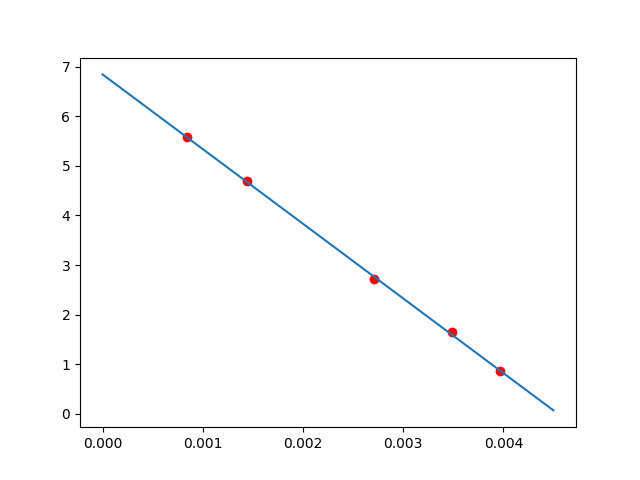
\includegraphics{Figure_1.png}
\end{adjustbox}

\section{Conclusões}

\subparagraph*{Os resultados foram dentro do esperado. O buffer de tensão manteve a tensão de saída igual a tensão de entrada.}

\subparagraph*{Algo que fiquei em dúvida foi sobre a resistência de Thévenin do buffer.}

\subparagraph*{A minha ideia eh montando o circuito com o buffer da seguinte maneira:}

\begin{center}
    \begin{circuitikz}
        \draw (0,0) to[battery1, invert] (0,3) to[resistor=$R_{th}$] (3,3) to[resistor=$R_L$] (3,0) -- (0,0);
    \end{circuitikz}
\end{center}

\subparagraph*{Teríamos que a tensão em $R_L$ é igual a tensão da fonte. Isto quer dizer que a resistência de thévenin do buffer é $0$ ?}



\end{document}